\textbf{If you enjoyed this book, you will enjoy\ldots}

\flushright

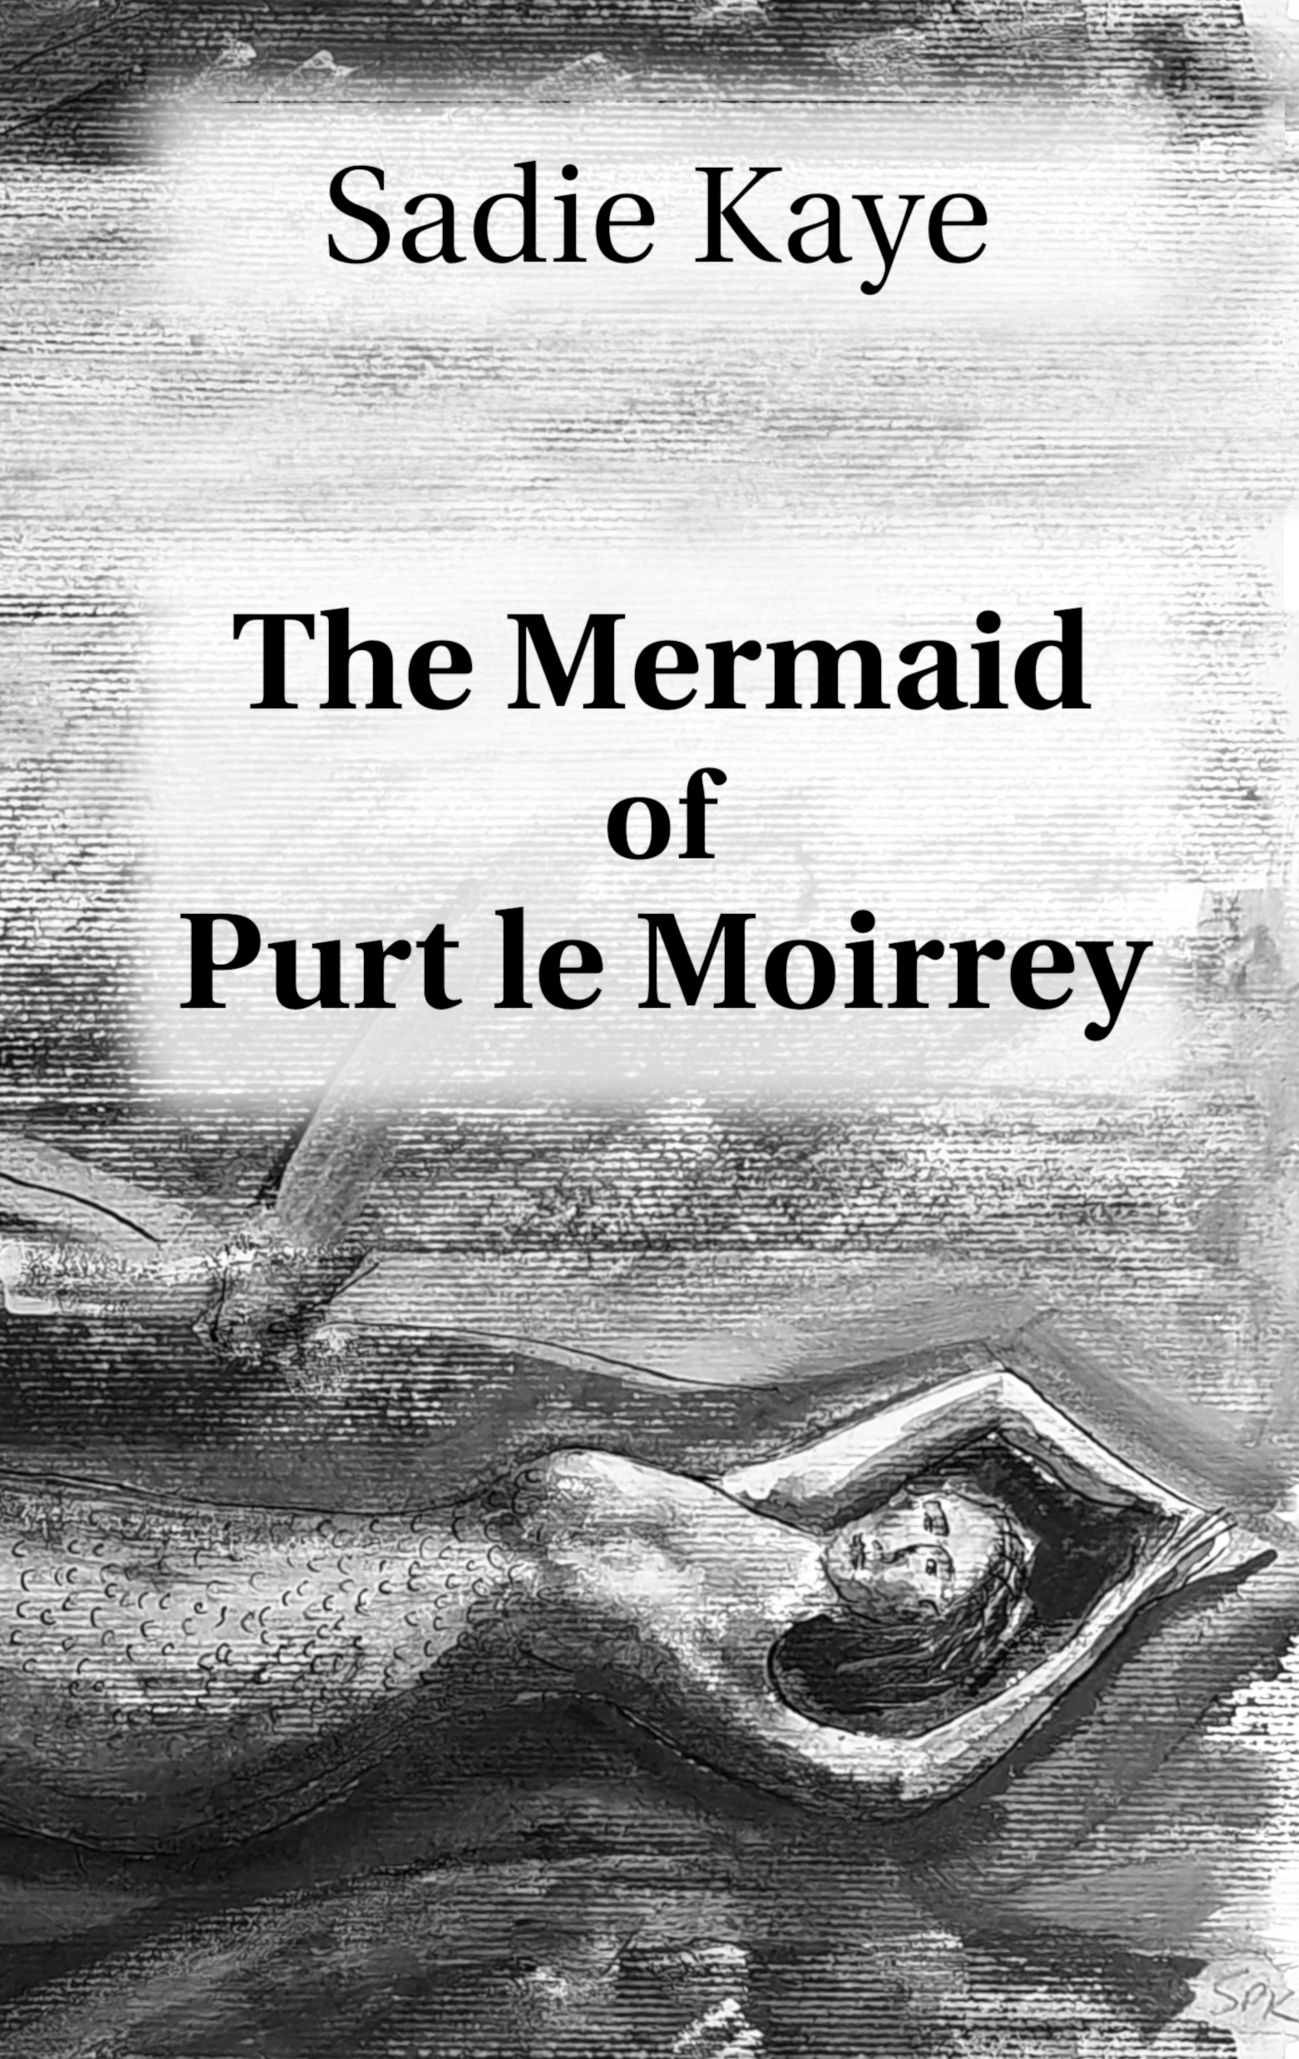
\includegraphics[width=0.58\textwidth]{mermaidcover.jpg}\hfill\parbox[b]{0.39\textwidth}{\tolerance 1000%
  %
  \textbf{The Mermaid of Purt le Moirrey,\\ by Sadie Philippa Kaye.}
  
  Samuel Collister is a poor fisherman from Purt le Moirrey (Port St Mary
  on the Isle of Man) who spots a mermaid at sea.  He follows her at sea
  and she brings him luck in his catch.  Their relationship blossoms into
  love but all is not well. Sam's mother and his fisherman friends are
  suspicious and jealous.
  
  \strut\qquad Always pointed and relevant to the modern day,
  this tale (written as a play in verse) provides a
  powerful reflection on\break
  \vskip -2.5ex%
  %
}\break
  % a
  % powerful reflection on
  love, prejudice and 
  courage to see beyond
  differences in marginalized communities.
  Paperback, 58 pages, illustrated with Sadie Kaye's pen and ink drawings.
  ISBN 978-1-914246-53-1.

  
`The Mermaid of Purt le Moirrey is a haunting and beautiful tale, part myth, part mirror, holding up the sea’s depths to our own hearts. Sadie Kaye weaves folklore into a powerful reflection on love, prejudice, and the courage to see beyond difference.' \textbf{Katie Victoria, author of: I write because\ldots}

`Updating an older fairy story put down by Dora Broome, Sadie how small-minded attitudes destroys lives and happiness.' \textbf{Jon Hartless, author of: Constructing Churchill}

  `Sadie eloquently gives a timeless myth of thwarted love modern resonance.'  \textbf{Lorna Rose, author of: Crown her with Ivy}
  
  \clearpage

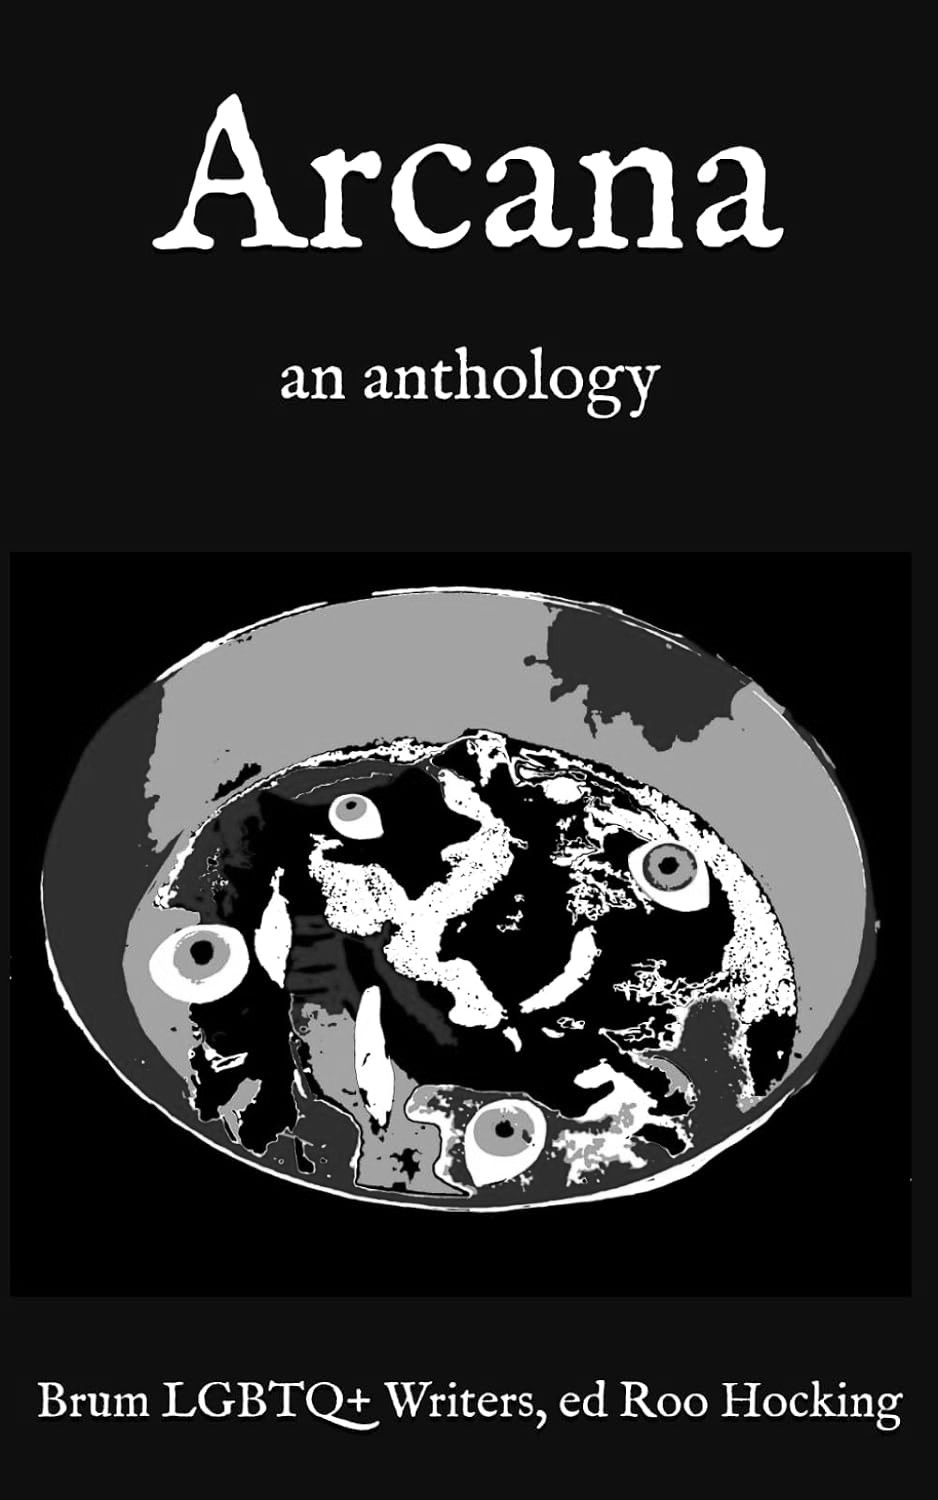
\includegraphics[width=0.48\textwidth]{arcanacover.jpg}\hfill\parbox[b]{0.49\textwidth}{\tolerance 1000%
  \textbf{Arcarna: an anthology, edited by Roo Hocking.}

  This richy illustrated anthology of new queer fiction gathers
  together twenty-two short, weird and fantastical pieces by
  Birmingham LGBTQ+ authors.  Together, they make up a new
  interpretation of the major arcana from the tarot, a curious blend
  of memory, fantasy and queer reality, with accompanying artwork by
  artist Kate Thompson.

   \strut\qquad What love story awaits the lunch-eater in the park?  Who might
   drink that Dolls Eye Soup?  And how long before her
   % dress goes up in flames?
}
dress goes up in flames?\\
  Paperback, 124 pages, ISBN 979-8319428752

  \medskip
  
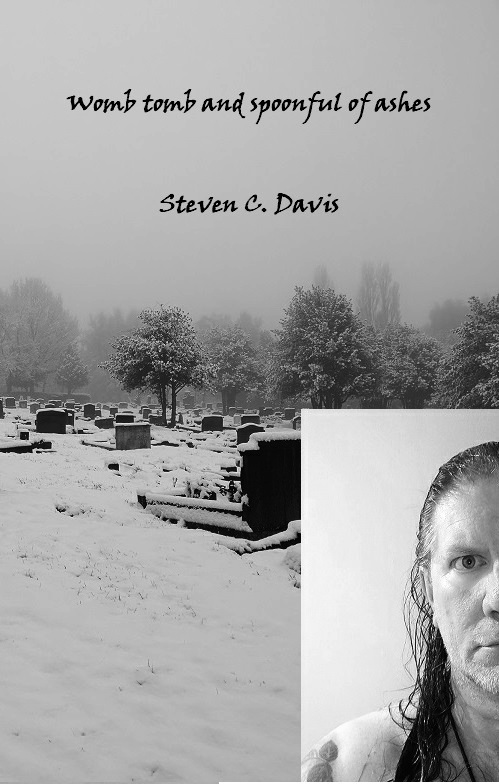
\includegraphics[width=0.48\textwidth]{wombtomb.jpg}\hfill\parbox[b]{0.49\textwidth}{\tolerance 1000%
  \textbf{Womb tomb and spoonful of ashes, by Steven C.~Davis}

A follow-up to Steven C. Davis' debut, 'Freshly dipped and bleeding
love', which was about transformation and change. This collection is
about life, death and everything in between, and quietly (and
sometimes not so quietly) rages. There are poems here about the
inequalities of the world, about being Ace, about god being a
Squirrel, about .. so much more. The underlying theme is unite. Whilst
you can achieve a lot on your own, you can achieve more
% if you join forces with others\ldots
}
if you join forces with others\ldots\\
Paperback, 68 pages, ISBN 978-1914246647 

\medskip

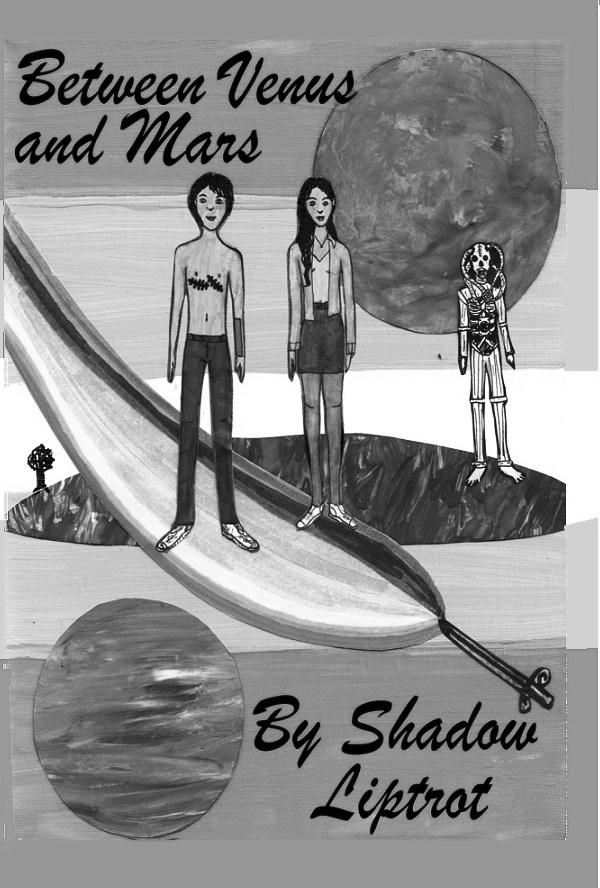
\includegraphics[width=0.48\textwidth]{VenusandMars.jpg}\hfill\parbox[b]{0.49\textwidth}{\tolerance 1000%
  \textbf{Between Venus and Mars, by Shadow Liptrot}
  
  How does it feel to be a trans man and unable to present as who you
  really are? It feels like you’re on a journey from Venus to Mars and
  you got trapped on Earth along the way. That is where Shadow
  Arlecchino is right now, except he is no longer physically on
  Earth. The president has sold humans into slavery. They have been
  put into gender camps and Shadow\=a trans man\=has been reassigned
  female.
  }
  His trauma is reawakened as he is forced to present as
  female again in order to survive. Is it worth it?

  How does it feel when the president of America sees human flesh as a
  sellable commodity? How does it feel when a writer you admired as a
  child betrays you and the entire LGBTQ+ community? How does it feel
  when aliens from the future are using AI to control everything we
  do?
  
  Paperback, 178 pages, ISBN 978-1914246630

\medskip

\medskip

\begin{center}
All available at Amazon.
\end{center}
